\documentclass[acmtog]{acmart}
\usepackage{graphicx}
\usepackage{subfigure}
\usepackage{natbib}
\usepackage{listings}
\usepackage{bm}
\usepackage{amsmath}

\definecolor{blve}{rgb}{0.3372549 , 0.61176471, 0.83921569}
\definecolor{gr33n}{rgb}{0.29019608, 0.7372549, 0.64705882}
\makeatletter
\lst@InstallKeywords k{class}{classstyle}\slshape{classstyle}{}ld
\definecolor{mygray}{rgb}{0.5,0.5,0.5}
\makeatother
\lstset{
 backgroundcolor=\color{lightgray}, 
 basicstyle = \footnotesize,       
 breakatwhitespace = false,        
 breaklines = true,                 
 captionpos = b,                    
 commentstyle = \color{mygreen}\bfseries,
 extendedchars = false,             
 frame =shadowbox, 
 framerule=0.5pt,
 keepspaces=true,
 keywordstyle=\color{blue}\bfseries, 
 language = C++,                     
 otherkeywords={string}, 
 numbers=left, 
 numbersep=5pt,
 numberstyle=\tiny\color{mygray},
 rulecolor=\color{black},         
 showspaces=false,  
 showstringspaces=false, 
 showtabs=false,    
 stepnumber=1,         
 stringstyle=\color{mymauve},        
 tabsize=2,          
 title=\lstname                      
}

% Title portion
\title{Assignment 3: {Ray Tracing Basics}} 

\author{Name:\quad WeiLiang Sun  \\ student number:\ 2020533010
\\email:\quad sunwl1@shanghaitech.edu.cn}

% Document starts
\begin{document}
\maketitle

\vspace*{2 ex}

\section{Introduction}

This is the assignment 3 of the computer graphics, finishing the following part:\\
\textbf{Part 1. Generate rays from camera} \\
\textbf{Part 2. Ray geometry intersection} \\
\textbf{Part 3. Phone lighting at intersection} \\
\textbf{Part 4. Light ray sampling for soft shadow} \\
\textbf{Part 5. Anti-aliasing by super resolution} \\
\textbf{Bonus Part 1. Texture mapping} \\
\textbf{Bonus Part 2. Normal/displacement texture} \\

\section{Implementation Details}

\subsection{Generate rays from camera}

In this part, we are taught to generate rays from the given camera. And two factors dx and dy are given, standing for the ray's location on raster space. Then with the help of dx and dy, we can calculate the coordinate in world space of this specific point. \\
We first normalize the raster space to a square with length one, to be more exact, [0,0] to [1,1]. \\
To calculate the up factor and right factor:(using the following formula)
$$up=focal\_len \cdot tan \frac{fov}{2}$$
$$right=aspect\_ratio \cdot focal\_len \cdot tan \frac{fov}{2}$$

Then in the class we know that the ray can be expressed as $r(t) = O+td$ where o is the original position and d is the direction. \\

Also we calculate the normal lookat function in this part: \\
\begin{lstlisting}
    forward = (look_at - position).normalized();
    right = forward.cross(ref_up).normalized();
    up = this->right.cross(this->forward).normalized();
\end{lstlisting}

\subsection{Ray geometry intersection}

\textbf{The first part: triangle}

In this part, we first assume some variables. Let the three vertexes of the triangle be $P_0$,$P_1$,$P_2$, the function of the ray is O+td where O is the origin position and d is the direction. \\
We combine two equations and we get the following equation: \\
$$o+td=(1-b_1-b_2)p_0+b_1p_1+b_2p_2$$
After changing the variables we get:
$$o-p_0=(p_1-p_0)b_1+(p_2-p_0)b_2-td$$
We let $E_1$ be $p_1-p_0$, $E_2$ be $p_2-p_0$, $S$ be $o-p_0$, then it changes to:
$$S=E_1b_1+E_2b_2-td$$
Using the formula we get:
$$t=\frac{det[S~E_1~E_2]}{det[-d~E_1~E_2]}$$
To calculate the numerator and the denominator:
$$det [-d~E_1~E_2]=-d \cdot (E_1 \cdot E_2)=E_1 \cdot(D\times E_2)$$
Let $S_1$ be $D\times E_2$, we get:
$$det [-d~E_1~E_2]=E1\cdot S_1$$
So to put everything in a nutshell, we get the t,$b_1$ and $b_2$:
$$t=\frac{S_2 \cdot E_2}{E_1 \cdot S_1}$$
$$b_1=\frac{S_1 \cdot S}{E_1 \cdot S_1}$$
$$b_2=\frac{S_2 \cdot d}{E_1 \cdot S_1}$$

\textbf{The second part: rectangle}

In this part, we consider the plane equation:$(P-P_0)\cdot n=0$ and the ray equation o+td. \\
After combining the two equations we get:
$$(o+td-P_0)\cdot n=0$$
So after judging whether intersection point is in the rectangle, we can compute dot product between $P-P_0$ and tangent or cotangent.\\
Also it is necessary to compare the dot product with size.x/2 and size.y/2.\\
Something about texture are also implemented in this function which will be described in following parts. 

\textbf{The third part: Ellipsoid}

In this part, there exists three matrixes. After calculating the three matrixes, we multiply these three matrix and get Matrix M. \\
Because M is the transform from unit sphere to ellipsoid, we also need to apply the inverse implementation to the matrix. \\
The judge condition can be calculated as following steps: \\
$$(o+td-c)^2-r^2 = 0$$
After changing the variables, we can get a equation. Using mathematics knowledge to calculate the $\delta$ we can get the condition:$d^2 <= 1.0f$

\subsection{Phone lighting at intersection}

\textbf{The first part: Evaluate radiance based on phone model}

In this part, we calculate all the hit light on the object by calculating the diffusion and specular based on phone lighting model. \\
To be more exact, all the things have been implemented in the last assignment.Diffusion is the light color times the surface color times the dot product of normal vector and the direction of incoming light. \\
Specular is the light color times the surface specular material times the dot product of viewing direction and reflection direction to the power of shiness.

\textbf{The second part: ray tracing with direct lighting}

In this part, we generate a ray through the center of pixel. Considering the condition if it intersects with any project. If it intersects with no objects in the scene, then it is considered as the fact that there is no light. The radiance under this condition should be set to zero. \\
If the ray intersects with the light, then it is considered as a light object. The radiance under this condition can be set to the color of its own light color. \\
If the ray intersects with an object such as triangle, rectangle or ellipsoid, we create a new ray from the intersection point to the light. To be careful, if there exists two intersection points, we choose the nearest one. If it intersect with geometry object, then it is shadowed, returning the ambient value. If it is rectangle, we can calculate the light color based on the phone lighting model, and then add all the radiance together to get the result. Of course, after the whole add, we should divide by the number of sampling points because the radiance of a pixel should be an average value instead of a value considering the value of number of sampling points. \\

\section{Light ray sampling for soft shadow}

In this part most of the contents are introduced in the part two of the last section. To be more exact, we judge if the ray is shadowed by the geometry object. If it is shadowed than return its ambient value, otherwise if it intersects with rectangle, add all radiance together to get the result color.

\section{Anti-aliasing by super-resolution}

In this part, we need to sample more than one ray to each pixel to realize the function of anti-aliasing. Also we know that the method of sampling all pixels can improve the render speed.\\
Of course, after we create the light sample, we should divide by the number of lights in the light sample to get an average result.

\section{Bonus part: Texture mapping}

\textbf{The first part: modifications in rectangle}

In the bonus part, we need to store two brand new variables named uv vector and model. uv vector is a vector used to show the position of the pixel in the texture map, so because the uv vector stands for a ratio, it needs to be set in range of 0 to 1. \\
In geometry rectangle: \\
We first find if the object should have material. Then we calculate the pos with the help of uv vector, translating the pixel position in texture map to our own scene position. After that, we have a function named get data to get the rgb of the pixel and multiply their factor such as tangent or cotangent. After the calculation, we get the final result of the interaction normal.

\textbf{The second part: anti-aliasing when texture is too small}

In this part, we need to consider the condition that the texture map is too big to hold the scene picture. In this part we use the method of bilinear interpolation. \\
In the interpolation part, we first get the four pixels around the given pixel, calculating the ratio of this pixel in the rectangle made up of the four round pixel. After that by using the ratio we can calculate the color of the given pixel. Implementing the method twice, and then divide by 255.f because of the rgb cause we can greatly solve the problem.

\section{Normal or Displacement texture}

In this part we need to deal with the normal texture and displacement texture. \\
Take the normal texture as example, we can know that when intersecting with a rectangle, it need to change its position due to the normal vector, to ensure the texture have some extend of normal.

\section{Results}
\begin{figure}[h]
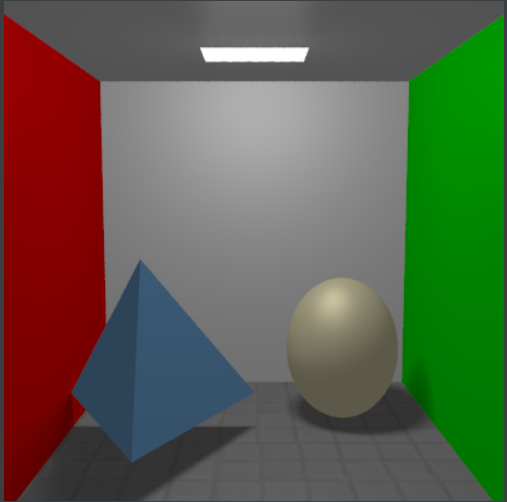
\includegraphics[width=4cm,height=4cm]{result}
\caption{the result picture}
\end{figure}

\end{document}